\section{Experiments}
\label{sec:eval}

\subsection{Evaluation design}
\label{sec:exp-design}
The runtime path throughout is \emph{runtime-safe}: every feature is computed
only from wire-observable telemetry, packets, and the defender's rated-capacity
model (Table~\ref{tab:provenance}); no feature reads attack ground truth. Real
QLoRA adapters (Qwen2.5-7B, Llama-3.1-8B; NF4 4-bit on one RTX~3080) run under
strict serving --- any run whose backbone or adapter is not loaded, whose
provenance is missing, or that would fall back to a heuristic, aborts. Ground
truth is used only by the offline evaluator after an action is chosen. The
unit of statistical inference is the \emph{configuration}; genuine stochastic
episodes are averaged within a configuration. Binary paired outcomes use the
exact McNemar test; continuous outcomes use paired sign-flip permutation tests
with paired bootstrap 95\% CIs and Cohen's $d_z$, Holm-corrected within each
hypothesis family; the permutation and bootstrap resampling draws are shared
across the contrasts of a family (common random numbers), so identical paired
difference vectors receive identical intervals; zero-event rates carry a
Clopper--Pearson 95\% upper bound.

Frozen assets, each hash-pinned before use: a canonical \textbf{70-case}
adversarial suite (14 families $\times$ 5 held-out cases per backbone,
leakage-controlled against the 200-example fine-tuning corpus --- zero exact or
normalized duplicates); a \textbf{32-configuration} Evidence-Gate test set plus
per-magnitude FDI probes; a hash-frozen \textbf{49-configuration} end-to-end holdout (33 attack across four families
plus fleet, 16 benign; two feeders; three episodes each) used for
system evaluation only; and a \textbf{12-configuration} estimator holdout for
counterfactual validation. A separate 25-configuration library is used for
development and threshold selection only, never for held-out reporting.
IEEE-123 is unavailable in the repository; the
holdout uses IEEE-13/34 and states the reduced feeder scope rather than
substituting.

\subsection{RQ1: does adversarial output reach an unsafe executable action?}
\label{sec:rq1}
\emph{Experiment.} Each of eight arms faces the canonical 70-case suite as
sustained input (eight ticks, so persistence-gated components fire), on the
runtime-safe architecture. The arms share the frozen case definitions, but
model generation is performed independently within each arm --- no arm
replays another arm's model output. Arm-level comparisons therefore
characterise complete-system behaviour and do not estimate a matched causal
effect on identical frozen model outputs. Per-decision provenance records the
model's proposal and the executed action separately; the denominator is the
adversarial case.

\emph{Result} (Table~\ref{tab:adv-v3-qwen}, Fig.~\ref{fig:containment-v3}). The
model is genuinely consulted --- it proposes a non-\textsc{no\_op} action --- on
$64/70$ cases (Qwen) and $70/70$ (Llama), so the containment below is the shield
acting on real proposals, not non-consultation. The unshielded model executes the
irreversible \textsc{isolate\_inverter} primitive on $61$ of $70$ cases (Qwen;
irreversible-execution rate $0.871$) and $18$ of $70$ (Llama; $0.257$); the
distinct, broader forbidden-action rate (any action in the case's must-not set)
is $46/70=0.657$ for Qwen. The full architecture,
and every ablation arm that retains the class-aware avoidance, executes it
\emph{zero} times (Clopper--Pearson 95\% upper bound $0.051$; policy violation
$0.000$). The independently executed arm without class-aware avoidance
exhibits $36$ of $70$ (Qwen) and $37$ of $70$ (Llama) executions (violation
$0.443$/$0.357$). The arm without the Evidence Gate shows unchanged
adversarial containment (still zero) --- the shield handles consulted
proposals regardless; the gate's role is benign-day selectivity (RQ2). The confidence-gated variant, which admitted an irreversible
action when model-stated confidence cleared a threshold, was \emph{worse than no
shield} ($0.743$ versus $0.657$ unshielded) because injection prompts manufacture that
confidence.

\emph{Interpretation.} Exactly one mechanism carries adversarial containment:
deterministic removal of unsafe actions, with irreversible proposals always
escalated. The consistency of the unshielded-model figure with an independent earlier
suite (61/70) is a cross-check on the harness. \emph{Limitation.} Marginal
contributions are measured against this suite; a component idle here may matter
elsewhere, and suite-bounded zeros are not universal guarantees.

\emph{Structural verification.} Because the 70-case suite only \emph{samples}
the danger, we additionally verify the shield structurally: we exhaustively
enumerate the discretised decision state space of the deterministic projection
--- $40{,}824$ combinations of evidence class, model proposal (including
out-of-registry and malformed output), stated confidence, severity, parse
status, and protocol-evidence hint --- and check every safety property at every
point. The executed action is always in the fixed registry, the irreversible
primitive is never executed autonomously (vetoed or escalated, never
executed), no class-inappropriate
action executes, a model stand-down never vetoes a deterministically evidenced
incident, and model failure always yields the deterministic fallback: $0$
violations over all $40{,}824$ points. Mutation tests confirm the properties are
load-bearing, not vacuous --- disabling the irreversible-escalation, class-aware
avoidance, or inaction-veto guard produces $1008$, $144$, and $3930$ violations
respectively. This is exhaustive over the modelled state space rather than a
sample from a real attack population.

\input{tables/final_v3/table_adversarial_v3_qwen}
\begin{table}[t]\centering\small
\caption{Canonical 70-case adversarial containment (llama), sustained input, observable-only runtime. Denominator = adversarial case ($n{=}70$). \emph{Irrev.\ prop.}\ and \emph{Irrev.\ exec.}\ are the irreversible-proposal and irreversible-\emph{execution} counts (action $=$ \texttt{isolate\_inverter}); \emph{Forbidden act.}\ is the distinct forbidden-action count (executed action in the case's must-not set). Zero-execution arms carry a two-sided Clopper--Pearson 95\% upper bound (\emph{exec.\ up95}). The correct-refusal rate and full per-arm metrics are in the supplementary material.}
\label{tab:adv-v3-llama}
\resizebox{\columnwidth}{!}{%
\begin{tabular}{lccccc}
\toprule
Arm & $n$ & Irrev.\ prop. & Irrev.\ exec. & exec.\ up95 & Forbidden act. \\
\midrule
Full arch. & 70 & 37/70 & 0/70 & 0.051 & 0/70 \\
$-$Evidence gate & 70 & 62/70 & 0/70 & 0.051 & 0/70 \\
$-$Projection & 70 & 37/70 & 0/70 & 0.051 & 0/70 \\
$-$Class avoidance & 70 & 37/70 & 37/70 & 0.649 & 25/70 \\
$-$Caution/HITL & 70 & 37/70 & 0/70 & 0.051 & 0/70 \\
$-$EH fallback & 70 & 37/70 & 0/70 & 0.051 & 0/70 \\
Deterministic only & 70 & 0/70 & 0/70 & 0.051 & 0/70 \\
Unshielded & 70 & 18/70 & 18/70 & 0.376 & 18/70 \\
\bottomrule
\end{tabular}}
\end{table}


\begin{figure}[t]
  \centering
  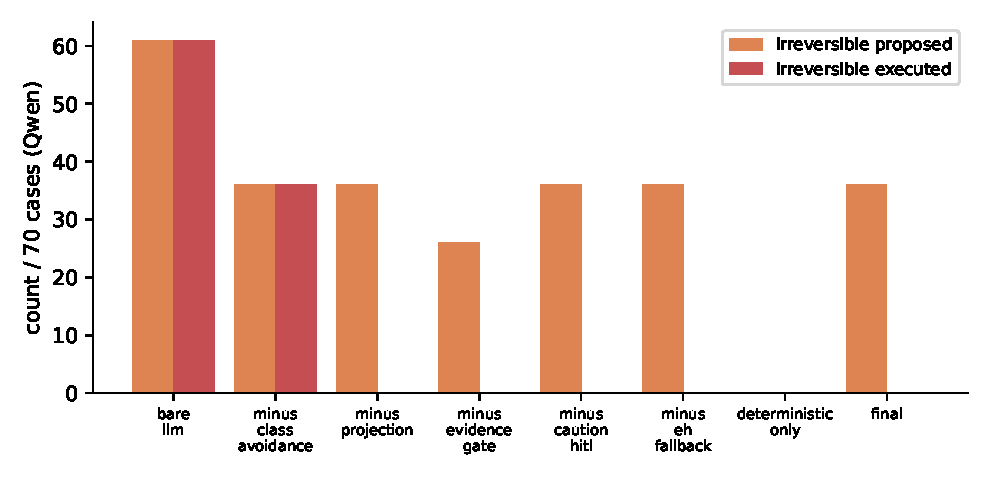
\includegraphics[width=0.95\columnwidth]{figure/final_v3/fig_containment_v3.pdf}
  \caption{Irreversible actions proposed versus executed per arm on the
    canonical 70-case runtime-safe adversarial suite (Qwen). Arms are
    executed independently on the shared frozen case definitions
    (\S\ref{sec:rq1}). The full architecture and every avoidance-retaining
    ablation arm execute zero; the arm without class-aware avoidance
    exhibits execution; the unshielded comparator executes 61/70.}
  \label{fig:containment-v3}
\end{figure}

\subsection{RQ2: does the gate reduce benign response yet retain incidents?}
\label{sec:rq2}
\emph{Experiment.} Gate thresholds are calibrated on development data and
hash-frozen before a one-shot evaluation on the 32-configuration test set plus
per-magnitude FDI probes, all runtime-safe. We report gate-open coverage per
family (did the gate fire during the attack --- a detector-side quantity,
distinct from downstream correct mitigation) and benign false-open, with
Clopper--Pearson intervals.

\emph{Result} (Table~\ref{tab:gate-v3}, Fig.~\ref{fig:gate-v3}). Under the
observable-only feature set, the tested gate rules opened in all four tested
configurations of each of command-spoof, replay (sequence regression), and DoS
(timestamp staleness) --- each $4/4$ --- and in the single tested above-capacity
FDI probe ($1/1$, caught by the rating-plausibility residual). These are small
samples and the Clopper--Pearson intervals (Table~\ref{tab:gate-v3}) remain wide;
they are not population-level detection estimates. Benign false-open is
$4/16 = 0.25$ $[0.07, 0.52]$, of which three of four are the historian-echo
protocol ambiguity. The honest cost is explicit: sub-capacity FDI is missed ($0/1$
medium, $0/1$ low) --- it has no observable hard signature and cannot be
separated from benign transients without redundant sensing, so we report FDI
coverage split by magnitude rather than as one number. On the 16 benign holdout
configurations, an exact McNemar test found no significant difference in
benign false-action between the deterministic path (D0) and the oracle-projection
arm (discordant pairs $4/0$, $p=0.125$). The gate's measured benefit is instead
that it cuts benign-day model consultations (\S\ref{sec:disc-timing}), bounding
the model's exposure to attacker-controllable prompt content.

\emph{Command evidence requires authentication.} A command packet on the
wire is not proof of an attack: a forged command and a legitimate DERMS
command are observationally identical unless the command is authenticated.
We make the distinction explicit (Table~\ref{tab:gate-auth}) by evaluating
command-spoof detection and benign \emph{legitimate authenticated command
bursts} under three policies. Treating any command as an attack detects the
spoof ($3/3$) but false-opens on every legitimate burst ($2/2$); requiring a
failed-authentication check detects the forgery ($3/3$) and does not
false-open ($0/2$); without authentication the command is \emph{UNKNOWN}
evidence and the gate can rely only on a separate protocol signature --- here
the duplicate-payload signature, which also false-opens because repeated
legitimate commands trip it. The lesson is that command-based detection is
sound only with authenticated command evidence or an explicit UNKNOWN
outcome routed to a human; we implement no cryptographic check and therefore
report command-spoof coverage under the observable-only regime as
conditional on this assumption.

\emph{Interpretation.} The tested gate rules detected the evaluated instances
that contained their prespecified observable protocol signatures (command-spoof,
replay, DoS); the fourth family (sub-capacity FDI) has no such signature and is
an observability limit, and command-based detection carries the authentication
caveat above. These are small tested samples, not population-level detectability
claims. \emph{Limitation.} The gate assumes an
instrumented protocol layer; a full DNP3/IEC-61850 sequence state machine
(reset, wrap, retransmission, session restart) and cryptographic
authentication are modelled only in part, and a stealthy attacker forging
internally consistent authenticated evidence is out of scope.

\begin{table}[t]
\centering\small
\caption{Evidence Gate detector-side coverage: per-group gate-open and benign
false-open on the hash-frozen 32-configuration test set plus per-magnitude FDI
probes, using only observable evidence. Thresholds calibrated on development
data and frozen before this evaluation. Two-sided Clopper--Pearson 95\%
intervals. Sub-capacity FDI (medium/low) has no observable hard signature and
is reported as a coverage miss.}
\label{tab:gate-v3}
\begin{tabular}{lccc}
\toprule
Group & $k/n$ & Rate & 95\% CI \\
\midrule
Benign false-open & 4/16 & 0.25 & [0.07, 0.52] \\
Gate-open command-spoof & 4/4 & 1.00 & [0.40, 1.00] \\
Gate-open DoS & 4/4 & 1.00 & [0.40, 1.00] \\
Gate-open FDI (high) & 1/1 & 1.00 & [0.03, 1.00] \\
Gate-open FDI (low) & 0/1 & 0.00 & [0.00, 0.97] \\
Gate-open FDI (med) & 0/1 & 0.00 & [0.00, 0.97] \\
Gate-open replay & 4/4 & 1.00 & [0.40, 1.00] \\
\bottomrule
\end{tabular}
\end{table}

\begin{table}[t]\centering\small
\caption{Command evidence requires authentication. Gate-open outcome for command-spoof attacks (forged, failed authentication) and benign \emph{legitimate authenticated command bursts}, under three command-evidence policies (three configurations each, any-episode aggregation). Only requiring a failed-authentication check both detects the forgery and does not false-open on legitimate commands; treating any command as an attack, or having no authentication (command evidence UNKNOWN, so only physical corroboration counts --- here the duplicate-payload of repeated legitimate commands), false-opens.}
\label{tab:gate-auth}
\begin{tabular}{lcc}
\toprule
Command-evidence policy & Spoof gate-open & Benign false-open \\
\midrule
Any command $=$ attack & 3/3 & 2/2 \\
Require failed auth. & 3/3 & 0/2 \\
Unauthenticated (UNKNOWN) & 3/3 & 2/2 \\
\bottomrule
\end{tabular}
\end{table}


\begin{figure}[t]
  \centering
  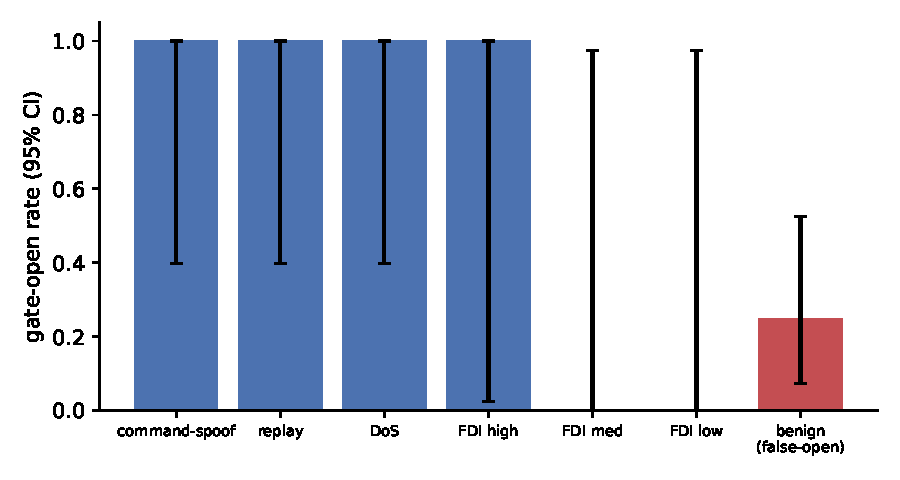
\includegraphics[width=0.82\columnwidth]{figure/final_v3/fig_gate_v3.pdf}
  \caption{Runtime-safe gate-open rate by attack family and benign false-open
    (95\% Clopper--Pearson intervals), using only observable evidence.
    Sub-capacity FDI (medium/low) is a documented observability miss.}
  \label{fig:gate-v3}
\end{figure}

\subsection{RQ3: what physical cost remains on an independent holdout?}
\label{sec:rq3}
\emph{Experiment.} The hash-frozen 49-configuration holdout (opened once, never
used for tuning) runs eight arms under the runtime-safe architecture with real
adapters: the deterministic fast path (D0); the ungated, fixed-cadence
model-only arms (ModelOnly-Q/L); the class-override shield (ClassOnly-Q/ClassOnly-L); the corrected projection
(SafeProj-Q/SafeProj-L) with irreversible-escalation, inaction-veto, and EH-ranked
fallback; and the oracle-class projection (OracleClass-Proj) as an evaluator-only upper
bound. Configuration is the inference unit.

\emph{Result} (Table~\ref{tab:holdout-v3}, Fig.~\ref{fig:holdout-v3},
Table~\ref{tab:stats-primary}). Zero serving fallbacks; adapters verified per
call. Mean attack ENS is D0 $0.352$, SafeProj-Q $0.537$, SafeProj-L $0.750$, ClassOnly-Q
$4.006$, ClassOnly-L $4.749$, ModelOnly-Q/L $8.484$, and OracleClass-Proj $0.067$.
The ModelOnly arms are \emph{diagnostic rather than matched shield ablations}:
they are ungated and poll the model on a fixed cadence that typically misses the
short attack window, so neither executes an effective mitigation in this holdout.
Their identical physical outcomes (byte-identical for ModelOnly-Q and ModelOnly-L,
both executing zero actions) therefore reflect the common unmitigated trajectory
rather than identical model behaviour, and their high ENS is \emph{not} a causal
estimate of shield removal --- shield use, evidence delivery, consultation
timing, and policy all differ at once. The evidence for unsafe unshielded
\emph{execution} is the adversarial result of \S\ref{sec:rq1}, where the model is
given the attack evidence directly. The projection arms show \emph{no
statistically detectable difference} from the deterministic path (SafeProj-Q
$+0.19$\,kWh, SafeProj-L $+0.40$\,kWh, both Holm $p=1.0$); no equivalence margin
was pre-registered, so we claim only the absence of a detectable difference, not
equivalence.
The ground-truth-class oracle is \emph{modestly better} than the deterministic
path (OracleClass-Proj$-$D0 $=-0.285$\,kWh, 95\% CI $[-0.69, -0.05]$, $d_z=-0.27$, raw
$p=0.015$; Holm-adjusted $p=0.11$, so the improvement does not survive
multiplicity correction across the primary family). We report this as a modest,
not-significant benefit rather than either ``no difference'' or a significant
gain: the bootstrap interval excludes zero while the adjusted test does not, a
distinction we make explicit. The LLM advisers do not reproduce even this
modest oracle benefit. Benign false-action is $0.062$ for the shielded model
arms against $0.25$ for the ungated deterministic path. That these conclusions
hold on prespecified, hash-frozen held-out configurations, under a runtime that
reads no attack ground truth, is the evidence they are not artefacts of a
strong detector.

\emph{Static OpenDSS power-flow plausibility check.} The 49-configuration
comparison uses the StubFeeder, a fast, stochastic simulation we treat as a
diagnostic rather than a deployment-validity result. To check that its physical
readings are plausible, we re-ran the deterministic and oracle-projection arms
through static OpenDSS IEEE-13/34 AC power-flow snapshots on the pre-registered
12-configuration subset, under the same observable-only runtime: all solves
converged (zero non-converged), and the two arms behave near-identically (mean
curtailment $17.6$ vs $17.7$\,kWh over the 11 attack configurations --- the
twelfth is the benign control --- and minimum voltage $0.975$\,pu). ENS is zero on
this subset because the feeders remain within the served-load envelope, so the
meaningful observed quantities are curtailment and voltage, not ENS. This is a
static snapshot check, not a dynamic quasi-static time-series study and not
real-feeder or utility validation; StubFeeder results remain simulation-based
diagnostic evidence. \emph{Limitation.} A dynamic quasi-static time-series study
across all arms is future work.

The estimator that ranks the shield's fallback set is validated separately
(Table~\ref{tab:eh-v3}): against branched counterfactual rollouts on the frozen
estimator holdout, the legacy 60-second estimator selects a tie-aware optimal
action in only a third of nominal configurations (top-1 $0.33$; $0.40$ averaged
over the ten robustness conditions) and carries large regret when it errs
(mean $76.3$\,kWh-eq), while the horizon-aware EH
selected a zero-regret action in all 12 tested held-out configurations and
retained that ranking under the evaluated perturbations (horizon misspecification
$\pm50\%$, delayed and partial execution, alternative cost weights). This result
reflects the coarse, structurally determined five-action ordering and the small
holdout; it should not be read as evidence of accurate impact-magnitude
prediction (MAE $\approx26$\,kWh) or of general real-feeder robustness, and we
make no magnitude-prediction claim.

\emph{Interpretation.} After containment, the residual physical cost of
consulting the model is small and is dominated by safe-but-suboptimal proposals
the shield honours inside the admissible candidate set --- a bounded, backbone-dependent cost the
admissible-set design, not the model, determines. \emph{Limitation.} StubFeeder and
static/quasi-static OpenDSS physics; the OpenDSS power-flow check
(supplementary material) is static, not dynamic.

\begin{table}[t]
\centering\small
\caption{Held-out end-to-end evaluation: 49 configurations (33 attack, 16
benign) $\times$ 3 stochastic episodes, observable-only runtime.
Configuration is the inference unit; episodes averaged within configuration.
\emph{Closed-loop coverage} is whether the incident is flagged at any tick of
the attack window in the closed loop; it is arm-dependent because each arm's
action feeds back into telemetry and the sustained-evidence gate (e.g.\ time to
first gate-open is $20$\,s for D0 vs.\ $111$\,s for L1), and is \emph{N/A} for
the ungated bare arms. It is \emph{not} the deterministic pre-action gate, which
is model-independent and identical across arms for identical input (verified:
$11{,}020$ pre-action ticks, $0$ violations); the detector-side gate recall is
Table~\ref{tab:gate-v3}. \emph{LLM calls} = sum over the 33 attack configs of
per-config mean calls (a sustained incident re-consults across ticks). Benign
false-action (FA) is physical-side. LLM arms run under strict serving (zero
fallbacks). Paired statistics in Table~\ref{tab:stats-primary}.}
\label{tab:holdout-v3}
\begin{tabular}{lcccccc}
\toprule
Arm & ENS & Curt. & Closed-loop & Benign & LLM & HITL \\
 & (kWh) & (kWh) & coverage & FA rate & calls & \\
\midrule
D0 & 0.352 & 11.52 & 0.949 & 0.250 & 0 & 0 \\
ModelOnly-Q & 8.484 & 17.05 & N/A & 0.000 & 66 & 0 \\
ModelOnly-L & 8.484 & 17.05 & N/A & 0.000 & 66 & 0 \\
ClassOnly-Q & 4.006 & 13.48 & 0.657 & 0.000 & 167 & 0 \\
ClassOnly-L & 4.749 & 13.84 & 0.657 & 0.062 & 167 & 0 \\
SafeProj-Q & 0.537 & 11.85 & 0.657 & 0.062 & 143 & 44 \\
SafeProj-L & 0.750 & 12.01 & 0.495 & 0.062 & 143 & 0 \\
OracleClass-Proj & 0.067 & 11.65 & 0.960 & 0.000 & 0 & 0 \\
\bottomrule
\end{tabular}
\end{table}

\begin{table}[t]
\centering\small
\caption{Primary paired configuration-level comparison on the held-out
49-configuration set: attack-window ENS difference of each arm minus the
deterministic fast path (D0), episodes averaged within configuration. Paired
bootstrap 95\% CI, Cohen's $d_z$, paired sign-flip permutation $p$, and
Holm-adjusted $p$ across this primary family; resampling draws are shared
across contrasts (common random numbers), so identical difference vectors
receive identical intervals (ModelOnly-Q/L). ``*'' marks Holm $p<0.05$. The
bootstrap CI can exclude zero while the adjusted test does not (OracleClass-Proj),
which we report as a modest, not-significant effect. ModelOnly arms are
diagnostic, not matched shield ablations (\S\ref{sec:rq3}).}
\label{tab:stats-primary}
\begin{tabular}{lcccccc}
\toprule
Contrast (ENS) & Mean diff & 95\% CI & $d_z$ & $N$ & $p_{\text{raw}}$ & $p_{\text{Holm}}$ \\
 & (kWh) & (kWh) & & cfg & & \\
\midrule
ModelOnly-Q$-$D0 & +8.133 & [+4.25, +12.46] & +0.66 & 33 & $<$0.001 & 0.008\,* \\
ModelOnly-L$-$D0 & +8.133 & [+4.25, +12.46] & +0.66 & 33 & $<$0.001 & 0.008\,* \\
ClassOnly-Q$-$D0 & +3.654 & [+1.31, +6.35] & +0.49 & 33 & 0.015 & 0.107 \\
ClassOnly-L$-$D0 & +4.398 & [+1.96, +7.12] & +0.57 & 33 & 0.005 & 0.041\,* \\
SafeProj-Q$-$D0 & +0.186 & [-0.62, +1.33] & +0.06 & 33 & 1.000 & 1.000 \\
SafeProj-L$-$D0 & +0.398 & [-0.47, +1.64] & +0.13 & 33 & 0.727 & 1.000 \\
OracleClass-Proj$-$D0 & -0.285 & [-0.69, -0.05] & -0.27 & 33 & 0.015 & 0.107 \\
\bottomrule
\end{tabular}
\end{table}


\begin{figure}[t]
  \centering
  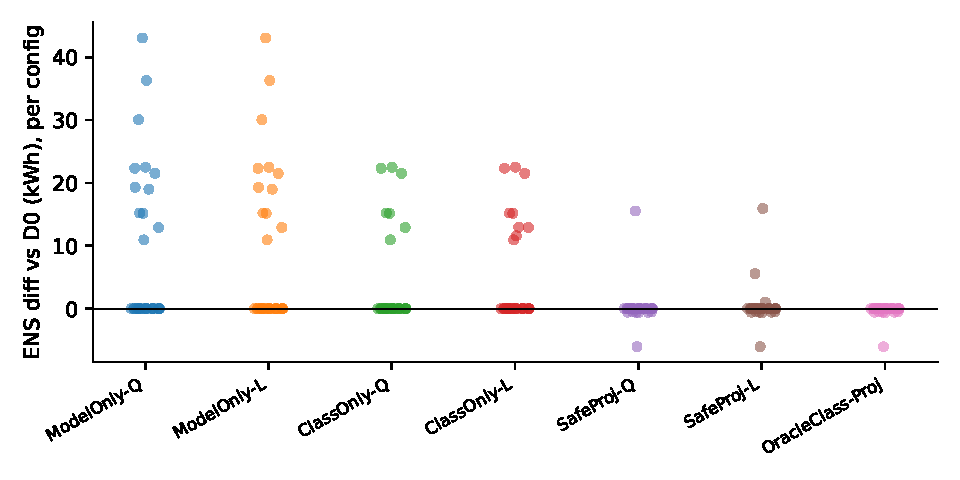
\includegraphics[width=\columnwidth]{figure/final_v3/fig_holdout_ens_diff.pdf}
  \caption{Per-configuration ENS difference versus the deterministic fast path
    (D0) on the independent 49-configuration holdout (paired CIs in
    Table~\ref{tab:stats-primary}). The projection arms (SafeProj-Q/SafeProj-L)
    sit near zero; the class-override arms sit above it; the ModelOnly arms
    (diagnostic, not matched ablations; \S\ref{sec:rq3}) sit highest.}
  \label{fig:holdout-v3}
\end{figure}

\begin{table}[t]
\centering\small
\caption{Horizon-aware estimator (EH) robustness: tie-aware top-1 optimal-action
rate and regret under horizon misspecification, delayed/partial execution, and
alternative cost weights, on the 12-configuration frozen estimator holdout. EH's
ranking is stable because the five-action choice is structurally determined;
point magnitudes remain imprecise (MAE $\approx$26\,kWh), so no
magnitude-prediction claim is made.}
\label{tab:eh-v3}
\begin{tabular}{lcccc}
\toprule
Condition & EH top-1 & EH med.\ regret & EH worst & E60 top-1 \\
\midrule
Nominal            & 1.00 & 0.00 & 0.0 & 0.33 \\
Horizon $-50\%$    & 1.00 & 0.00 & 0.0 & 0.33 \\
Horizon $-25\%$    & 1.00 & 0.00 & 0.0 & 0.33 \\
Horizon $+25\%$    & 1.00 & 0.00 & 0.0 & 0.33 \\
Horizon $+50\%$    & 1.00 & 0.00 & 0.0 & 0.33 \\
Delayed 10\,s      & 1.00 & 0.00 & 0.0 & 0.33 \\
Delayed 30\,s      & 1.00 & 0.00 & 0.0 & 0.33 \\
Partial failure    & 1.00 & 0.00 & 0.0 & 1.00 \\
$w_{\text{ENS}}=3$ & 1.00 & 0.00 & 0.0 & 0.33 \\
$w_{\text{ENS}}=8$ & 1.00 & 0.00 & 0.0 & 0.33 \\
\bottomrule
\end{tabular}
\end{table}


\subsection{RQ4: does the safety boundary hold under latency and fallback?}
\label{sec:rq4}
\emph{Experiment.} In deadline-aware mode the deterministic fast path acts at
detection; the model runs concurrently and its action replaces the fast-path
action only if it arrives within the service-level objective and passes every
safety check; an expired result never rewrites history. Measured per-call
latencies (Table~\ref{tab:latency-v3}) are replayed at SLOs of $1$--$60$\,s.

\emph{Result.} Single-call ($K{=}1$) inference is $5.45$\,s mean (Qwen) /
$5.62$\,s (Llama); $K{=}3$ self-consistency is $16.8$--$17.4$\,s and is not the
default. All latency values in the paper are regenerated from one measurement
file (Table~\ref{tab:latency-v3}). At a $1$\,s SLO no consultation lands
and the fast path stands alone; $K{=}1$ admits from $10$\,s (Qwen $0.99$, Llama
$1.00$), $K{=}3$ only from $30$\,s. Because the shield maps any accepted
proposal onto the same bounded primitive, physical outcomes are unchanged across
SLOs, and a late or failed model call deterministically leaves the fast-path
action in force under invariant~I5 (tested, not formally proved).
\emph{Interpretation.} The fast-path/slow-path split is an implementation-feasible
posture in the evaluated testbed: the model is advisory, and its absence
never removes containment. \emph{Limitation.} Latencies are single-GPU;
utility-grade serving changes constants, not the architecture.

\begin{table}[t]
\centering\small
\caption{Per-backbone, per-$K$ consultation-latency distribution, from the
146-call ($K{=}1$) / 48-call ($K{=}3$) measurements; single-call ($K{=}1$)
inference is $\approx$5.5\,s on both backbones. All latency values in the paper
are regenerated from this measurement file. Adapter load is a one-off startup
cost, not part of per-call latency.}
\label{tab:latency-v3}
\begin{tabular}{llccccccc}
\toprule
Backend & $K$ & $n$ & mean & median & s.d. & p95 & p99 & max \\
 & & & (s) & (s) & (s) & (s) & (s) & (s) \\
\midrule
Qwen & $K{=}1$ & 146 & 5.45 & 5.51 & 0.90 & 6.22 & 8.60 & 11.76 \\
Qwen & $K{=}3$ & 48 & 16.82 & 17.41 & 1.47 & 18.32 & 19.06 & 19.14 \\
Llama & $K{=}1$ & 146 & 5.62 & 5.60 & 0.57 & 6.56 & 7.03 & 8.34 \\
Llama & $K{=}3$ & 48 & 17.45 & 17.54 & 1.65 & 20.25 & 22.28 & 23.60 \\
\bottomrule
\end{tabular}
\end{table}

